\documentclass[12pt]{jsarticle}
\usepackage[dvipdfmx]{graphicx}
\usepackage{listings}
\lstset{
  basicstyle={\ttfamily},
  identifierstyle={\small},
  commentstyle={\smallitshape},
  keywordstyle={\small\bfseries},
  ndkeywordstyle={\small},
  stringstyle={\small\ttfamily},
  frame={tb},
  breaklines=true,
  columns=[l]{fullflexible},
  numbers=left,
  xrightmargin=0zw,
  xleftmargin=3zw,
  numberstyle={\scriptsize},
  stepnumber=1,
  numbersep=1zw,
  lineskip=-0.5ex
}             
\begin{document}

\section{コード規約}
プログラムを書いて機能を実装するだけというのは、内容が短くかつ一人で管理する際には対応できるかもしれないが、複数人でかつ長期的に保守・運用するときには、コードを書くだけでなく、他の人にもコードがよみやすくする配慮が重要になってくると考える。そのなかでも、コーディング規約はを守って書くかということは、その見やすさの客観的な指標になりうると思うので、1つものトピックとしては、「コーディング規約」を取り上げる。

講義を受ける前にも{}の位置や演算子の前後には空白を入れるといった、いくつかのコード規則は学んだこともあり、知っていることもあったが、この講義を通してまだ学べていなかったコード規則についても学ぶことができた。

実際に、講義内で学んだことであると、引数が複数行に渡るときのインデントの書き方や、演算子の前で改行するか演算子の後で開業するかといった議論は納得するところもあり、曖昧にしてしまっていた部分でもあったので勉強になった。

また、コードのチェッカーやフォーマッタをVScode内に導入していなかったこともあり、VScode内に flake8とautopepを導入して設定を行った上で、自動保存によりコードのフォーマットを整えられるようにした。これまでは、コードフォーマットを整えようと意識している反面、全てに気を配ることは難しく統一感が薄れてしまう部分もあったが、実際にこれらの拡張機能を追加し活用していくことで、読みやすいコードを意識しつつ統一性のあるコードを書けるようになっていると感じる。

次は、実際に今回のレポート用にいくつかの関数を作成し、それらをPEP8のコード規約に従うように実践したのでそれについてまとめる。これらは演習だけではなく、実際に各トピックの実践を行うことでより活用できるように考えている。

下記のコードでは、後述するgithub上にtips.pyとしてあげている私がよく使うコードを関数化したものである。コード規約にのっとって考えると、演算子の前後に空白を加えることだったり、","の後に空白を加えることは注意して書くべきところであるが注意して書き、コードフォーマッタで、最終的なチェックを行った。

下記のプログラムで実装した関数は以下の3つ。
\begin{itemize}
  \item current\_date : 現在の日付を出力する関数
  \item read\_csv     : csv を読み込む関数 (.csv の省略)
  \item to\_csv\_date  : csv を書き出す関数 ( 日付つきのファイル名 )
\end{itemize}

下記の例では、コード量が少ないこともあり、PEP8のコード規約を十分に実践できたわけではないが、他のプログラムも書いていく過程で複数行に渡るコードを書く場合には曖昧にしてしまうと迷ってしまうことが多い。そのような中でPEP8の規則を学びそれらを実践することで統一性があり、可読性の高いコードを書くことができると感じているので今回はその練習として実践できてよかったと感じる。また、学びきれなかったコード規則もあると思うので、勉強していきたいと感じるとともに、プロジェクトの開発チームごとにも従うべきコード規則というものがそれぞれあると感じるので、基礎を整えた上でそれらにも柔軟に対応できるようにしていきたいと思う。

\begin{lstlisting}[caption=tips.py]
import pandas as pd
import datetime

# 現在の日付を出力する関数
def current_date():
    dt_now = datetime.datetime.now()
    dt_now_format = dt_now.strftime('%Y%m%d')
    return dt_now_format

# csv を読み込む関数 (.csv の省略)
def read_csv(df_name):
    return pd.read_csv(df_name + ".csv")

# csv を書き出す関数 ( 日付つきのファイル名 )
def to_csv_date(df, filename):
    df.to_csv(filename + '_' + current_date() + '.csv')

\end{lstlisting}

\newpage
\section{ドキュメンテーション}
前の課題では、コード規約について取り上げたが、今回のトピックもコード規約と同じく、自分がコードを書いたときに人に読んでもらいやすくするために必要な「ドキュメンテーション」について取り上げる。

コード規約にのっとったコードを書いて読みやすくなったとしても、他の人が書いたコードを1からすべてに目を通して理解するといったことは現実的ではない。実際にライブラリを使うときにライブラリの実装コードをすべて見て理解してから使うのでは効率的とは言えない使い方になってしまう。そのようなときに、関数ごとにまとめられたドキュメントがあると、使いたい関数の検索性も高まり、理解したい部分を効率的に理解できるなど重要性を強く感じることができる。さらに、コード中に組み込むことで関数間の関係性も維持したまま、抜け漏れがなく書ける工夫もとても興味深く重要なものであると感じた。

\subsection{コメント}
コメント一つをとっても、良いコメントと悪いコメントが存在する。私も漠然と他の人が書いているコードを読みながら意識していたところでもあったが、それらが文面上で講義内では示していただいていて、納得できるとともに今後のコメントを書く上での指針にしようと感じた。実際にそのコードが行っている処理内容に関して記述するのであれば、1行ずつコードを読んでいくことと大差ない。その一方、そのコードが存在する理由を書くことで、コードのかたまりとしての概観をつかむことができるので、可読性をあげることができると感じる。

\subsection{docstring}
ドキュメントを作成するということは、リファレンスマニュアルを作ることになるが、関数名とその機能、引数と返り値をはじめとした使用例といった、関数やクラスの仕様を説明するためのコメントとして、docstring というものがある。これらの基本要素は決まっているので、VScodeにはそれを自動生成する Python Docstring Generatorがあり、この講義を通して知ったので、実際に導入してこのレポートで後述するドキュメント作成にも活用した。このように、フォーマットが決まっていることによって、関数によって説明する内容がばらばらになるということを防ぎ、統一感の説明をしやすくできるという点で重要であるといえる。

\subsection{ドキュメント作成ツール}
ドキュメントをコードと別々に作成していては、作業量が倍になるだけではなく、一方の更新や作成のし忘れが起こりやすくなってしまう。そこで、コード内に書いたコメントからドキュメントを生成するツールとして、Doxygen と Sphinx があげられる。

Doxygenは、C/C++を用いた開発を部活で行っていた際に使っていたため、知っているが、コード内にコメントとして加えるだけでhtmlが作成されプログラム外からその関数の特性や、探したい関数を見つけやすくなった点で、一覧性と検索性の2点から優れていたと感じる。しかし、毎回 @ からはじめなければいけない点はコードを書く上で煩雑さを感じた。

次に、Sphinxについてはこの講義で名前については知ったが、スライドを見たらドキュメントで良くみたことのある形式であり、それらのライブラリがSphinxで書かれていたことを知りSphinxの人気の高さを実感した。コメントとしても、前述の拡張機能と合わせて最小限のコードで書くことができるようにも感じる。

\subsection{Sphinx を用いた実践}
前課題につづいて、自作した3つの関数についてのドキュメントをSphinxを用いて生成を行ったところ図\ref{fig:sphinx}のように生成することができた。Sphinxを使ったことは講義前はなかったが、実際に使ってみて使いやすさを感じたので、今後の自分が関わるプロジェクトでもこのようにドキュメントを作成していき、共有しやすくできるようにしたいと感じた。(これらのコード,htmlに関しても後述するgithubにpushしている)

\begin{figure}[htbp]
  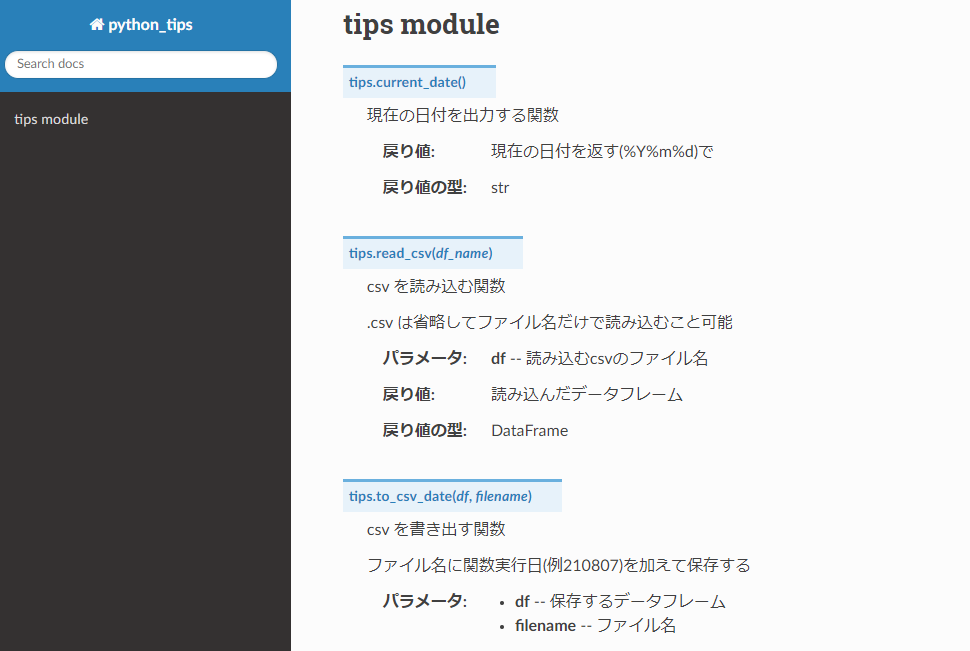
\includegraphics[width=6.0cm]{./sphinx.png}
  \caption{Sphinxを用いた自作関数のドキュメント}
  \label{fig:sphinx}
\end{figure}



\newpage
\section{バージョン管理・GitHub}
\subsection{バージョン管理}


\subsection{Git VScode拡張機能}


\subsection{Github}


\subsection{Github 実践}


\newpage
\section{コンテナ管理}

\end{document}
